%----------------------------------------------------------------------------------------
%	PACKAGES AND DOCUMENT CONFIGURATIONS
%----------------------------------------------------------------------------------------

\documentclass[11pt]{article}

\usepackage[english]{babel}
\usepackage[utf8]{inputenc}
\usepackage[T1]{fontenc}
\usepackage[top=3cm, bottom=3cm, left=2.5cm, right=3.5cm]{geometry}
\usepackage{graphicx}
\usepackage[babel=true]{csquotes} % csquotes va utiliser la langue définie dans babel

\setlength\parindent{0pt} % Removes all indentation from paragraphs

\begin{document}

\begin{center}
\begin{large}
\textsl{LifeBand : How to set up the application} \\
\end{large}
.............................................................. \\
\end{center}

\paragraph{} Thank you for pilot testing the LifeBand application. This guide explains how to set up the app in only five small steps.

\begin{tabular}{p{3.5cm}p{12cm}}
\begin{center}
Fig. 1
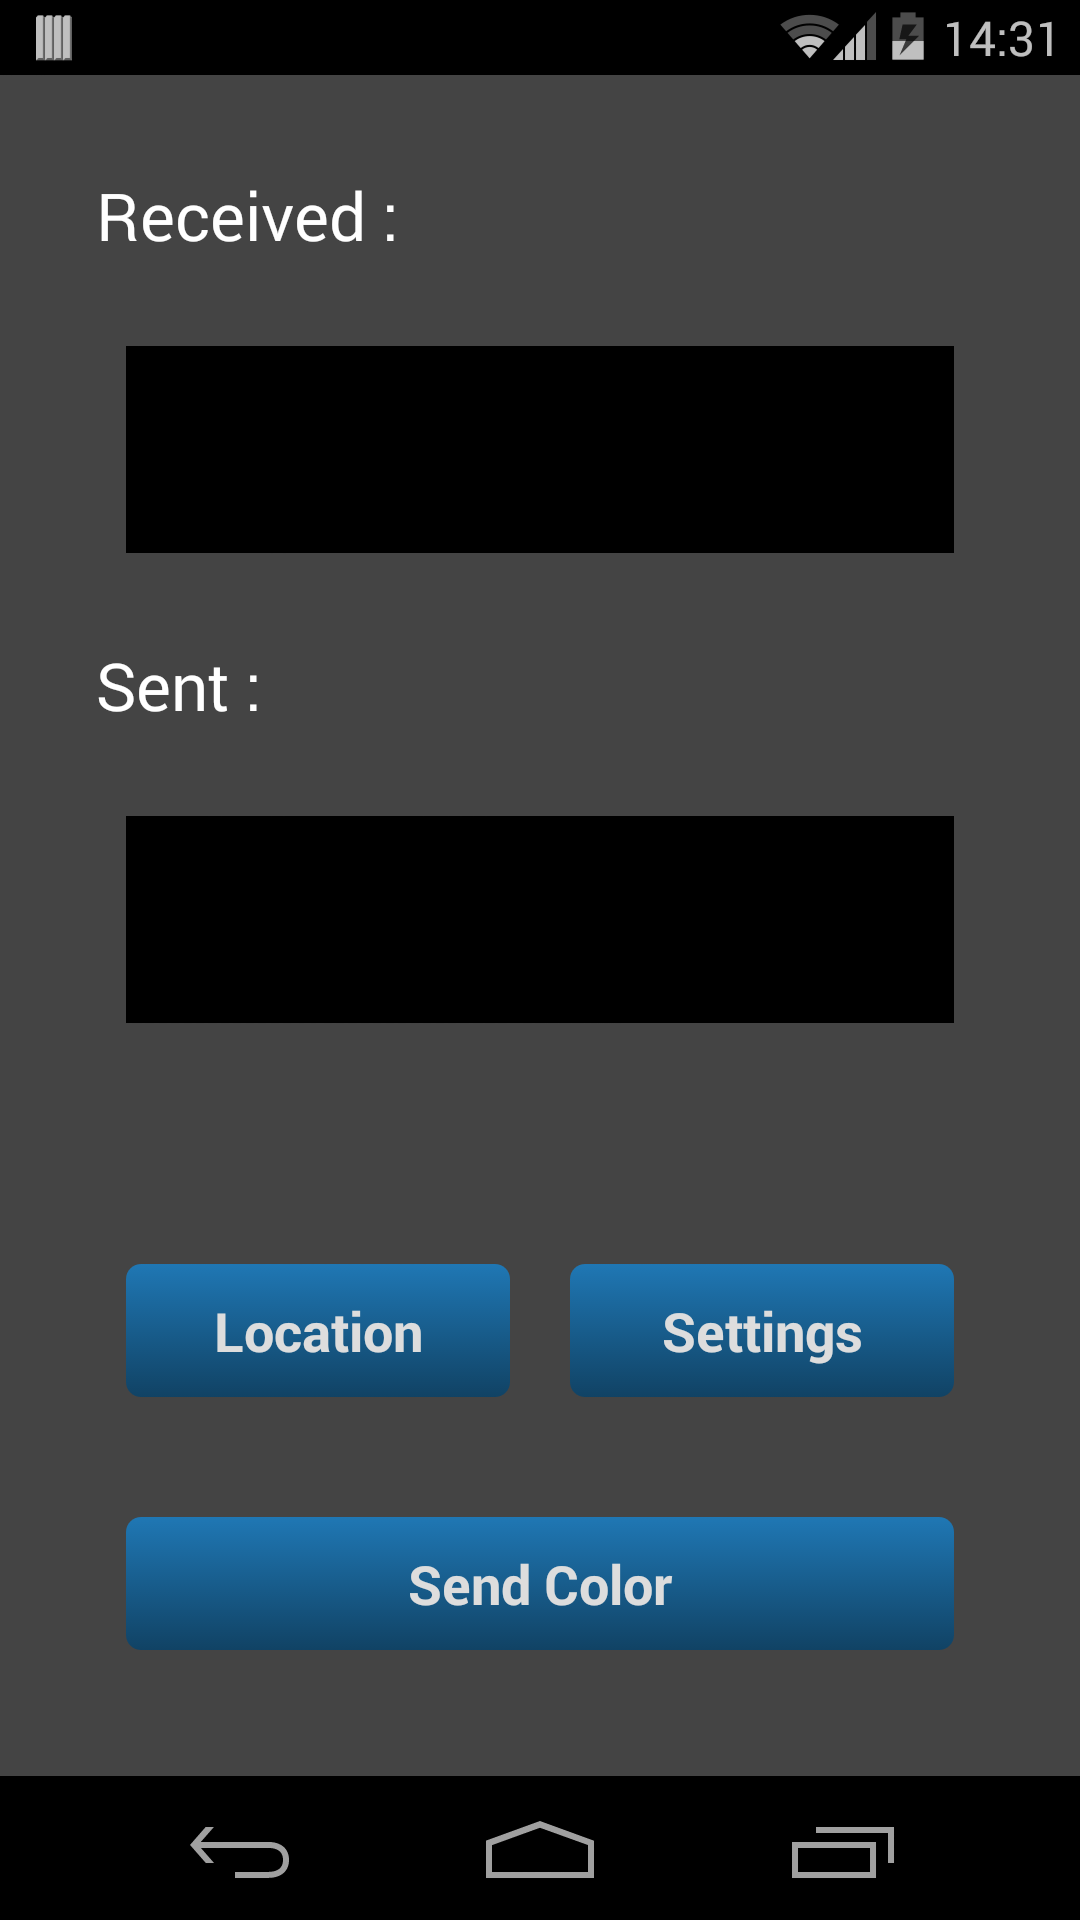
\includegraphics[width=2.8cm]{home.png}\newline
Fig. 2
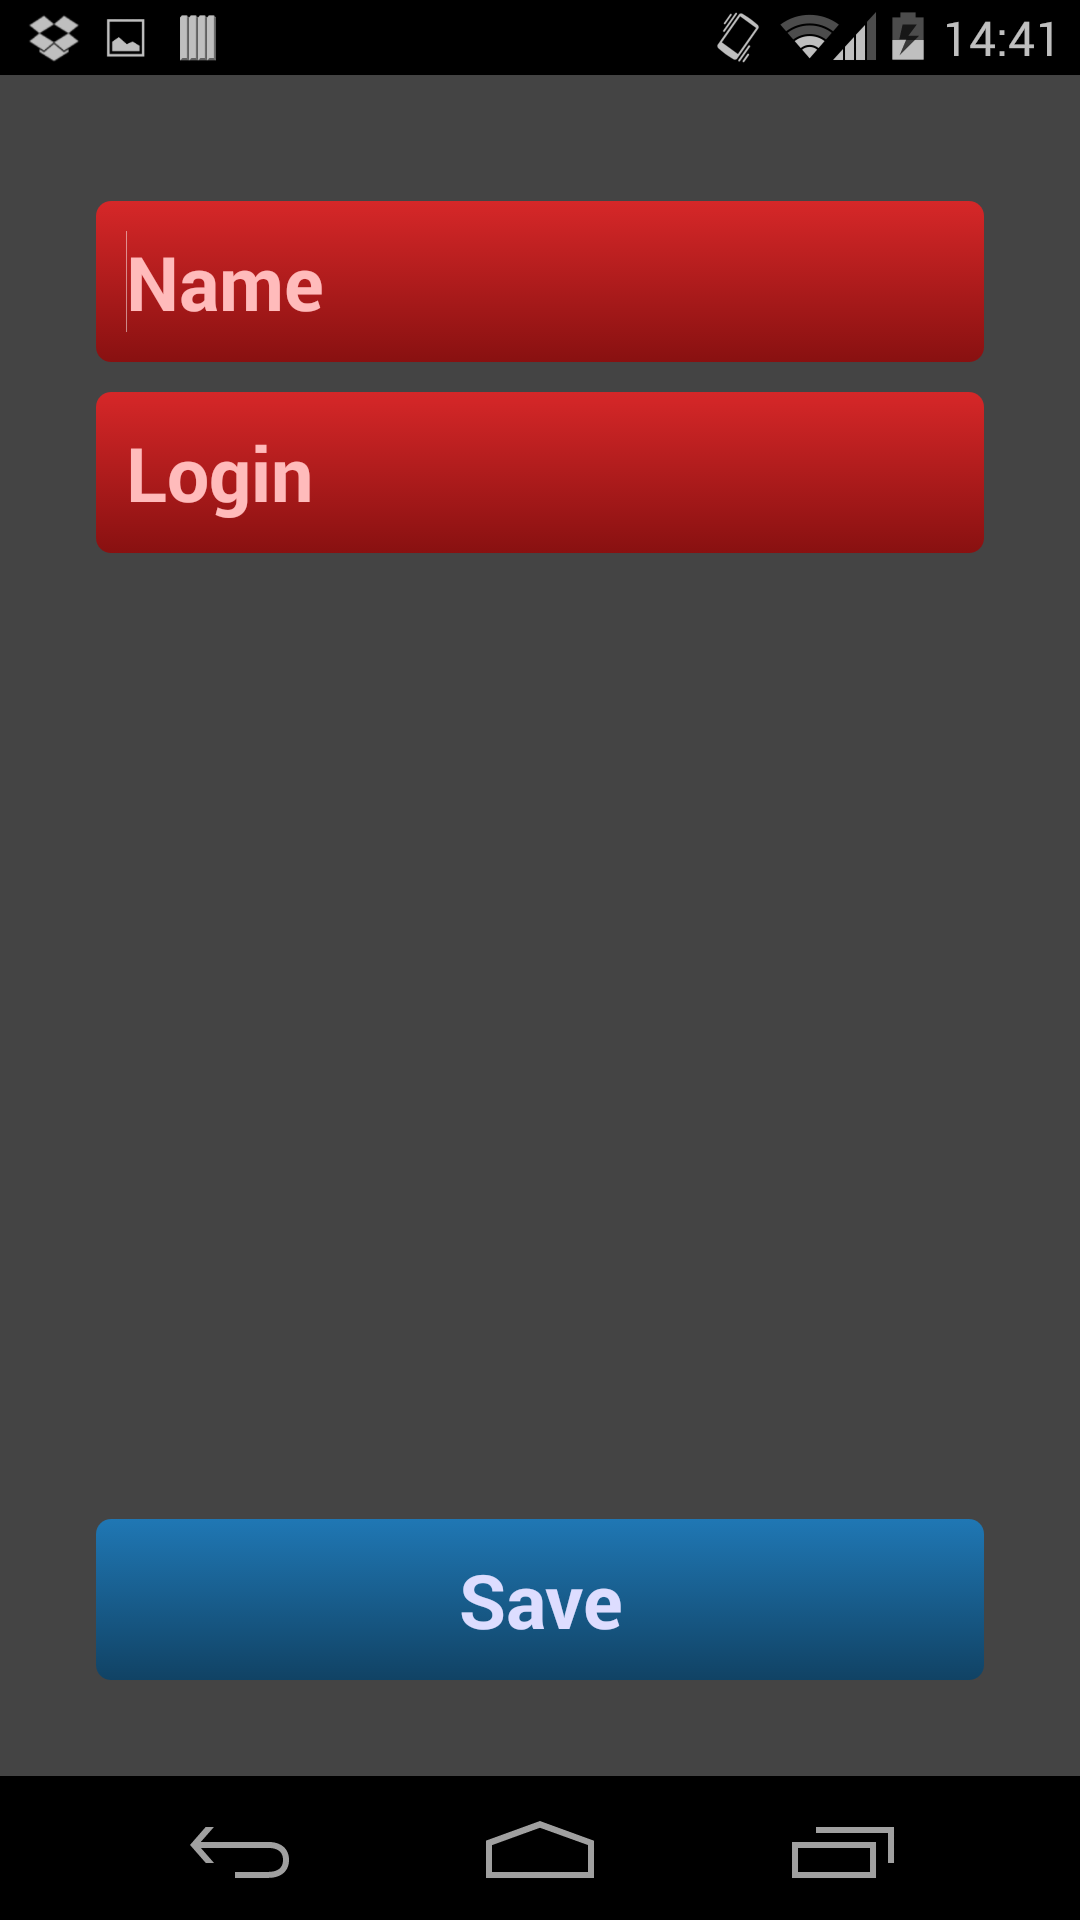
\includegraphics[width=2.8cm]{user.png}\newline
Fig. 3
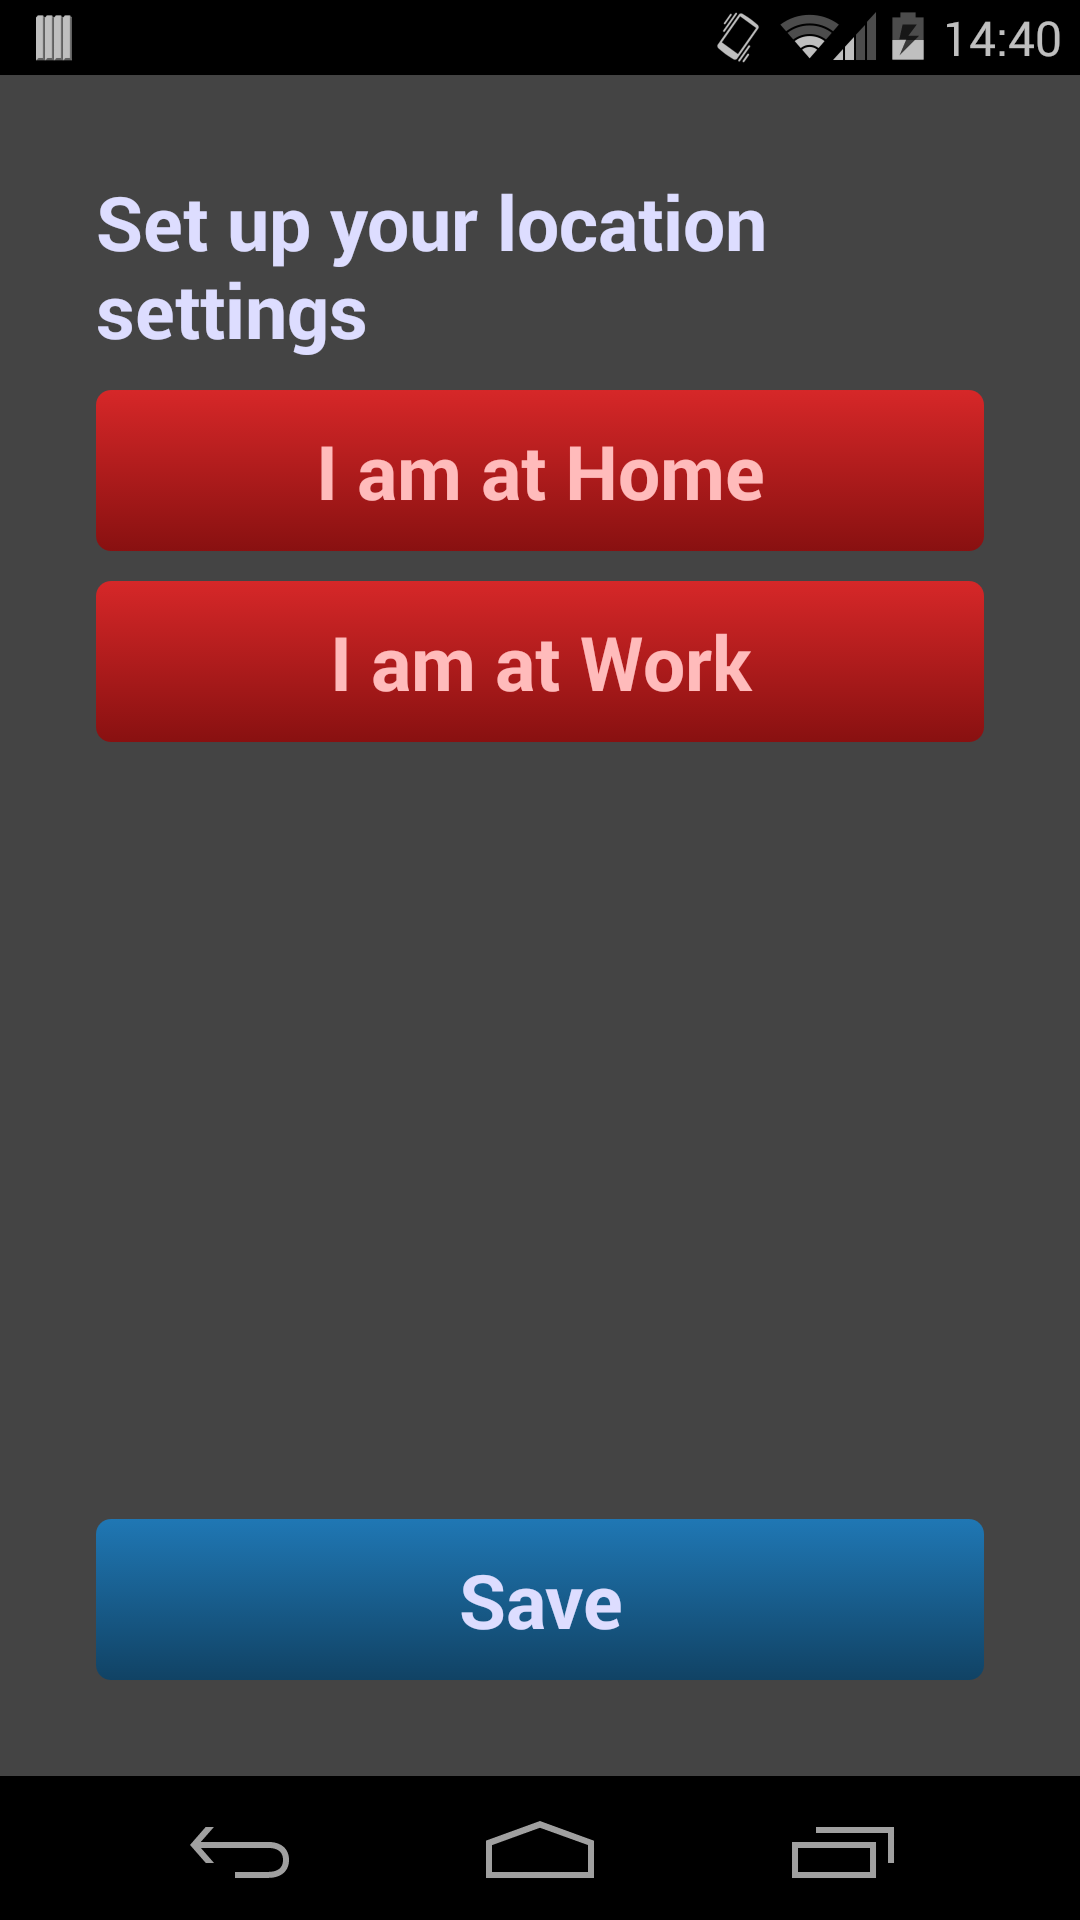
\includegraphics[width=2.8cm]{location.png}\newline
\end{center}
&
\paragraph{Step 1 : Install the app}
\paragraph{} Download the apk file and copy it on your smartphone. You can either download it on your computer and use a cable or open on your smartphone the link I sent you by email. Once the apk file is copied on your smartphone, you just need to click on it. The installation will require that you authorize installation from unknown sources. For security reason you might want to unauthorize again just after installing the app.

\paragraph{Step 2 : Launch the app}
\paragraph{} The app is called LifeBand, you just need to find it among all your other apps. You should see the first screen (Fig. 1) when launching it.

\paragraph{Step 3 : Fill in personal information}
\paragraph{} Click on the "Settings" button (Fig. 1) to access to the personal information screen (Fig. 2). You must fill in your first name and choose a login that must be the same for you and your partner. Then click on the "Save" button.

\paragraph{Step 4 : Fill in location information}
\paragraph{} Click on the "Location" button (Fig. 1) to access the location information screen (Fig. 3). To set it up, you must define where your home and work places are. To do this, click once on "I am at Home" and "I am at Work" when you are at each location. You can redefine these places as many times as you want.

\paragraph{Step 5 : Add the widget to your home screen}
\paragraph{} Find it among your other widgets and place it on your phone home screen. \\
\end{tabular}


\vfill
\begin{center}
.............................................................. \\
Université Paris Sud - LRI - in|situ|
\end{center}

\end{document}